\documentclass[a4paper,12pt]{article}
\usepackage{fontspec}
\usepackage{polyglossia}
\setmainlanguage{russian}
\setotherlanguage{english}

\usepackage{amsmath}
\usepackage{amssymb}
\usepackage{geometry}
\usepackage{graphicx}
\usepackage{hyperref}
\usepackage{fontspec}
\usepackage{xcolor}
\usepackage{minted}
\usepackage{fvextra}
\usepackage{tikz}
\usepackage[normalem]{ulem}

\usemintedstyle{trac}
% \usemintedstyle{material}

\geometry{top=2cm,bottom=2cm,left=2cm,right=2cm}

\setmainfont[Path = ./fonts/]{centuryschoolbook.ttf}
\newfontfamily\cyrillicfont[Path = ./fonts/]{centuryschoolbook.ttf}
\newfontfamily\cyrillicfontsf[Path = ./fonts/]{centuryschoolbook.ttf}
\newfontfamily\cyrillicfonttt[
    Path = ./fonts/,
    UprightFont = *-Regular.ttf,
    ItalicFont = *-Italic.ttf,
    BoldFont = *-Bold.ttf,
    BoldItalicFont = *-BoldItalic.ttf
]{AdwaitaMono}

\setmonofont[
    Path = ./fonts/,
    UprightFont = *-Regular.ttf,
    ItalicFont = *-Italic.ttf,
    BoldFont = *-Bold.ttf,
    BoldItalicFont = *-BoldItalic.ttf
]{AdwaitaMono}

\title{Алгоритмы и структуры данных}
\author{densine}
\date{\today}

\begin{document}

\maketitle
\tableofcontents

\section{От автора}
Этот документ я делаю торопясь, поэтому если вдруг вы найдете ошибки или же недостатки -
просто пишите мне в ЛС в Telegram - @Denantm. Я всегда рад исправлениям и стоящим
советам по написанию документов и т.п. Начнем.

\section{Организационные моменты}

\subsection{Платформа, контесты, оценки...}
Все занятия будут проходить на платформе algocourses.ru, логины для каждого контеста можно
найти в файле в канале параллели (пароли те же, что и от аккаунта, в котором вы писали
отборочный этап).
Ваши старания и усилия будут оцениваться, и в зависимости от их результата, вы можете получить
стипендию или перейти в другую параллель (стипендии у параллели С нет уж точно).
Оценка рассчитывается примерно так:
\[
Rate = 0.7 * ContenstRate + 0.3 * TestRate + 0.1 * ExamsRate
\]

Затем, если ваша оценка  $>=7$ - вас не исключают и вы продолжаете заниматься (информация
неподтверждена).

На уроки в дистанционном формате ссылка будет появляться в канале паралелли.

\section{Введение}
На этом курсе изучаются основы C++ для решения олимпиадных задач. Цели - научить
решать подобные задачи на С++ и подготовить в региональному этапу Всероса по информатике.
(Слова не мои, это было на сайте). В введении разберем общие для олимпиадного
программирования понятия - O-нотацию и основы С++.

\subsection{Оценка сложности алгоритмов - O-нотация}
Для начала разберемся, как мы оцениваем сложнось того или иного алгоритма.
Универсальной для нас единицой измерения будет количество операций.
Например:
\begin{itemize}
\item если мы суммируем два числа - $a$ и $b$, например, то совершается 1 операция.
\item если наш алгоритм суммирует числа от 1 до n:
\[
1 + 2 + ... + n - 1 + n = ...
\]
То всего будет совершено n - 1 Операций.
\item если наш алгоритм суммирует все числа в матрице n на n:
\[
X =
\begin{matrix}
x_1 & x_2 & \dots & n \\
x_{n+1} & x_{n+2} & \dots & x_{2n} \\
\vdots & \vdots & \ddots & \vdots \\
x_{n*(n-1)} & ... & ... & x_{n^2} \\
\end{matrix}
\]
то совершается $n^2 - 1$ операций.
\end{itemize}
Или же, используя код на Python:
\begin{minted}
[
    tabsize=4,
    frame=single,
    framesep=2mm,
]
{python}
print(a + b) # 1 операция

sum_of_1_to_n = 1
for i in range(2, n + 1): # n - 1 операций
    sum_of_1_to_n += i # 1 операция

# Итого - n - 1 операций.

sum_of_1_to_n_squared = 0
for i in range(n): # n операций
    for j in range(1, n + 1): # n операций
        sum_of_1_to_n_squared += i * n + j # 1 операция

# n*n = n^2 операций.
\end{minted}

Затем, сама асимптотическая сложность записывается как $O(...)$, где внутри
скобок оставляем только самое быстрорастущее значение, а константы опускаем. Напимер:
\begin{itemize}
\item Возьмем строчку
\mint{python}|print(a + b)|
$a + b$ - одна операция, но для наглядности скажем, что и $print(...)$ выполняется за
несколько операций. Тогда сложность - $O(1)$, после того, как опустим константы.
$1$ в $0$ превратить нельзя - тогда $n$ превращалось бы в $0$, как и любая другая переменная.
\item Рассмотрим второй цикл. Выполняется он за $n - 1$ операций, после того,
как опустим константы - $O(n)$.
\item Теперь рассмотрим код целиком! Суммарная сложность - $1 + n + n^2$. Выбираем
самый значимый элемент - в нашем случае $n^2$ - и опускаем константы. Получаем $O(n^2)$
\end{itemize}

Вопрос - зачем нам вообще нужно оценивать сложность алгоритма? Компьютер все-таки имеет
свои лимиты, а сервер на олимпиаде уж точно, и оценить их тоже можно в количестве выполняемых
операций, например, в секунду. Так, если ограничение по времени выполнения - 1 секунда,
а сложность нашей программы на Python - $O(n^2)$, то скорее всего появится ошибка Time Limit Exceeded
(или что-то в этом духе) - время исполнения превышено, так как язык вроде Python выдерживает
$\sim5*10^8$ операций в секунду. Т.е. максимальный n - $sqrt(5*10^8)\approx22000$. Поэтому важно
оптимизировать алгоритмы, а понять, до какой степени это нужно делать поможет асимптотическая
сложность.

\subsection{Основы С++}
Здесь я, по понятным причинам, описывать все прикасы и уродства всеми любимого
С++ не буду, для этого есть отдельные уроки или курсы. Сами организаторы "Алгоритмов и
структур" советуют \href{https://stepik.org/course/363/syllabus}{этот курс}, лично
я советую хендбук Яндекса - там много задач связанных
с теми или иными фичами языка.

\subsection{Контейнеры}
Контейнер - это тип, позволяющий хранить в себе объекты других типов (списки и т.д.).
С vector'ом вы познакомитесь как с основой С++, но несколько других полезных контейнеров
мы разберем, реализуя с помощью него. Представляем вам стек, очередь, и деку! Разберем
по порядку.

\begin{itemize}
\item Стек - структура last in - first out (последний зашел, первый вышел - LIFO).
Пример из жизни: стопка блинов. Когда вы их готовите, последний кладете (по крайней мере,
обычно) сверху, а когда едите - берете тоже сверху.

В С++ есть структура $stack$, однако мы рекомендуем использовать вместе нее $vector$.
Методы, которые должен реализовывать стек:
\begin{minted}
[
    tabsize=4,
    frame=single,
    framesep=2mm,
]
{cpp}
#include <vector>
...
std::vector<T> stack;

stack.push_back(elem); // Добавить элемент на вершину стека
stack.pop_back();      // Удалить верхний элемент стека
stack.size()           // Размер стека
...
\end{minted}
Что мы можем сделать, чтобы найти минимум в стеке? Вызывать функции вроде $min$ каждый раз
неэффективно (они могут иметь сложность до $n$). Взамен этого мы можем поддерживать стек
с текущими минимумами! Каждый раз, когда мы добавляем элемент в стек, сравниваем его с последним
элементом стека минимумов, и если он меньше - добавляем его, иначе добавляем снова последний
элемент стека минимумов.
Рассмотрим пример. Пусть наши входные данные выглядят так:
\[
x = [5, 2, 3, 4, 1]
\]
и мы имеем два стека:
\begin{minted}{c++}
std::vector<int> stack;
std::vector<int> minsstack;
\end{minted}
Рассмотрим каждый добавленный элемент и как выглядит стек в этот момент.

\begin{enumerate}

\item $x_1 = 5$. Оба стека пусты, значит просто добавляем в конец каждого стека $x = 5$:

\begin{minted}{cpp}
stack.push_back(x);
minsstack.push_back(x);
\end{minted}
$stack = [5]$; $minsstack = [5]$

\item $x_2 = 2$. Сравниваем последний элемент $minsstack$ с $x = 2$ и добавляем меньшее
из $x_1 = 5$ и $x_2 = 2$, т.е. \uline{правую часть} std::min(...):

\begin{minted}[escapeinside = ||]{cpp}
stack.push_back(x);
minsstack.push_back(std::min(minsstack.back(), |\ttfamily\uline{x}|));
\end{minted}
$stack = [5, 2]$; $minsstack = [5, 2]$

\item $x_3 = 3$. Текущий $x$ больше последнего элемента $minsstack$, значит добавляем не
$x$, а последний элемент $minsstack$, т.е. \uline{левую часть} std::min(...):

\begin{minted}[escapeinside = ||]{cpp}
stack.push_back(x);
minsstack.push_back(std::min(|\ttfamily\uline{minsstack.back()}|, x));
\end{minted}
$stack = [5, 2, 3]$; $minsstack = [5, 2, 2]$

\item $x_4 = 4$. $x_4 > x_2$, значит в конец minsstack добавляем $x_2$.
$stack = [5, 2, 3, 4]$; $minsstack = [5, 2, 2, 2]$

\item $x_5 = 1$, $x_5 < x_2$, значит в конец minsstack добавляем $x_5$.
$stack = [5, 2, 3, 4, 1]$; $minsstack = [5, 2, 2, 2, 1]$
\end{enumerate}

Таким образом получается стек обычный и стек префиксных минимумов. Затем, если нам
нужно удалить последний элемент стека, мы просто удаляем его из обоих стеков:

\begin{minted}[frame=single, framesep=2mm]{cpp}
stack.pop_back();
minsstack.pop_back();
\end{minted}

\item Следующая структура - очередь (queue). Для нее характерна концепция "первым зашел,
первым вышел" - first in-first out (FIFO). В C++ есть готовая структура:
\begin{minted}[frame=single, framesep=2mm]{cpp}
#include <queue>
...
std::queue<T> queue;
queue.push(elem); // Добавить элемент в конец очереди
queue.pop();      // Удалить элемент из начала очереди
queue.size();     // Узнать размер очереди
queue[i]          // Получть i-ый элемент очереди
\end{minted}

Также очередь можно реализовать с помощью двух стеков. Покажем на примере:
Для начала, пусть у нас есть два стека - left и right.
\mint{cpp}|std::vector<int> left; std::vector<int> right;|
Чтобы добавить элемент в конец очереди:
\mint{cpp}|right.push_back();|
А чтобы удалить... нам нужно проверить, пуст ли стек $left$:
\begin{itemize}
\item если пуст - мы переносим все элементы из правого стека в левый, причем последний
элемент правого становится первым левого. Затем, просто удаляем последний элемент
левого стека:
\begin{minted}[frame=single, framesep=2mm]{cpp}
...
while (!right.empty()) {
    left.push_back(right.back());
    right.pop_back();
}

left.pop_back();
...
\end{minted}
\item иначе - просто удаляем последний элемент левого стека.
\end{itemize}

На вопрос "Почему это работает, как положено" можно ответить графически:

\begin{center}
    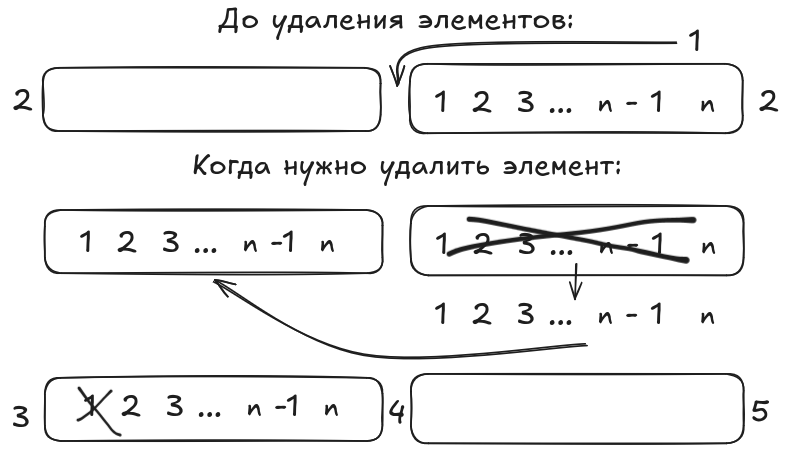
\includegraphics[width=0.7\textwidth]{assets/queue with 2 stacks.png}
\end{center}

Пояснения:
\begin{enumerate}
\item Ради удобства иллюстрации, начало обоих стеков находится по центру...
\item ...а концы - по краям, т.е. левый стек идет от центра к левому краю, а правый -
от центра к правому краю.
Получается, что очередь визуализировать очень просто можно с помощью
двух стеков с пераметрами (1-2). Тогда:
\item начало очереди, если левый стек непуст
\item начало очереди, если левый стек пуст
\item всегда конец очереди. Это означает, что для того, чтобы добавить элемент в конец
очереди нужно просто добавить его в конец правого стека.
\end{enumerate}

Зачем нужна очередь из двух стеков? Для того, чтобы находить ее минимум. Реализацию
поддержки минимума здесь оставлять не буду, просто скажу, что нужно поддерживать минимум
обоих стеков.

\item Последняя изученная нами сегодня структура - дека (dequeue). По сути это совмещение
и очереди, и стека - элементы можно добавлять и убирать с обоих сторон. Эту структуру
можно реализовать с помощью стеков, но их потребуется 5+ штук, поэтому мы просто используем
встроенную в С++ ее реализацию.
\begin{minted}[frame=single, framesep=2mm]{cpp}
#include <deque>
...
std::deque<T> deque;
deque.push_front(elem); // Вставить элемент в начало деки
deque.push_back(elem);  // Вставить элемент в конец деки
deque.pop_front();      // Удалить элемент из начала деки
deque.pop_back();       // Удалить элемент из конца деки
deque.size();           // Узнаить размер деки
...
\end{minted}

\end{itemize}

Это все контейнеры, что были разобраны на лекции. Отмечу, что все они реализуют методы
.back() и .front(), возвращающие ссылки на последний и первый элементы этих структур,
а также .end() и .begin() - итераторы, указывающие на ячейки после и до структур (удобны
для получения -2, -3 т.д. элементов).

\end{document}
